% Created by tikzDevice version 0.7.0 on 2014-07-31 11:04:27
% !TEX encoding = UTF-8 Unicode
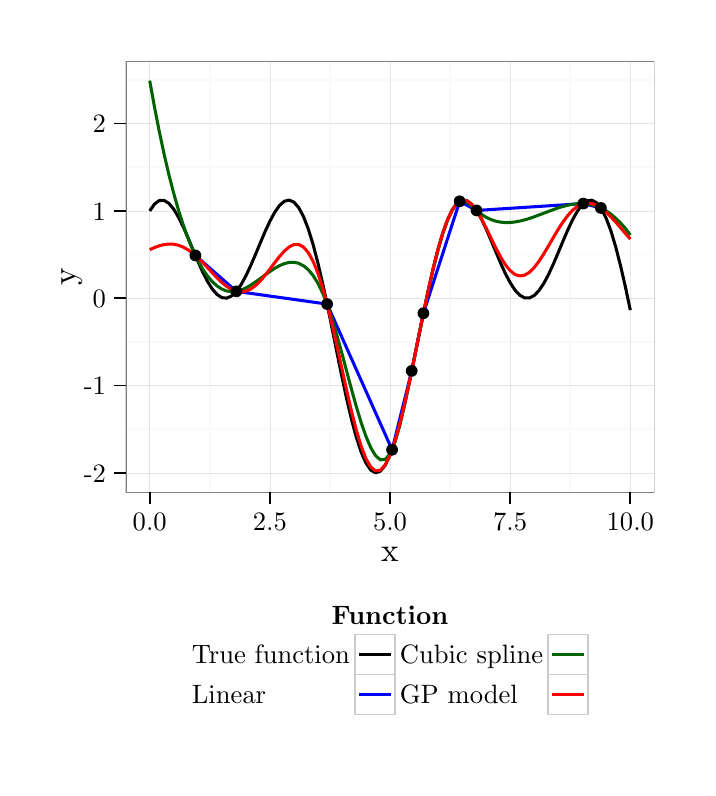
\begin{tikzpicture}[x=1pt,y=1pt]
\definecolor[named]{fillColor}{rgb}{1.00,1.00,1.00}
\path[use as bounding box,fill=fillColor,fill opacity=0.00] (0,0) rectangle (238.49,267.40);
\begin{scope}
\path[clip] (  0.00,  0.00) rectangle (238.49,267.40);
\definecolor[named]{drawColor}{rgb}{1.00,1.00,1.00}
\definecolor[named]{fillColor}{rgb}{1.00,1.00,1.00}

\path[draw=drawColor,line width= 0.6pt,line join=round,line cap=round,fill=fillColor] (  0.00,  0.00) rectangle (238.49,267.40);
\end{scope}
\begin{scope}
\path[clip] ( 35.42, 99.45) rectangle (226.45,255.35);
\definecolor[named]{fillColor}{rgb}{1.00,1.00,1.00}

\path[fill=fillColor] ( 35.42, 99.45) rectangle (226.45,255.35);
\definecolor[named]{drawColor}{rgb}{0.98,0.98,0.98}

\path[draw=drawColor,line width= 0.6pt,line join=round] ( 35.42,122.30) --
	(226.45,122.30);

\path[draw=drawColor,line width= 0.6pt,line join=round] ( 35.42,153.85) --
	(226.45,153.85);

\path[draw=drawColor,line width= 0.6pt,line join=round] ( 35.42,185.39) --
	(226.45,185.39);

\path[draw=drawColor,line width= 0.6pt,line join=round] ( 35.42,216.94) --
	(226.45,216.94);

\path[draw=drawColor,line width= 0.6pt,line join=round] ( 35.42,248.49) --
	(226.45,248.49);

\path[draw=drawColor,line width= 0.6pt,line join=round] ( 65.81, 99.45) --
	( 65.81,255.35);

\path[draw=drawColor,line width= 0.6pt,line join=round] (109.23, 99.45) --
	(109.23,255.35);

\path[draw=drawColor,line width= 0.6pt,line join=round] (152.64, 99.45) --
	(152.64,255.35);

\path[draw=drawColor,line width= 0.6pt,line join=round] (196.06, 99.45) --
	(196.06,255.35);
\definecolor[named]{drawColor}{rgb}{0.90,0.90,0.90}

\path[draw=drawColor,line width= 0.2pt,line join=round] ( 35.42,106.53) --
	(226.45,106.53);

\path[draw=drawColor,line width= 0.2pt,line join=round] ( 35.42,138.07) --
	(226.45,138.07);

\path[draw=drawColor,line width= 0.2pt,line join=round] ( 35.42,169.62) --
	(226.45,169.62);

\path[draw=drawColor,line width= 0.2pt,line join=round] ( 35.42,201.17) --
	(226.45,201.17);

\path[draw=drawColor,line width= 0.2pt,line join=round] ( 35.42,232.71) --
	(226.45,232.71);

\path[draw=drawColor,line width= 0.2pt,line join=round] ( 44.10, 99.45) --
	( 44.10,255.35);

\path[draw=drawColor,line width= 0.2pt,line join=round] ( 87.52, 99.45) --
	( 87.52,255.35);

\path[draw=drawColor,line width= 0.2pt,line join=round] (130.93, 99.45) --
	(130.93,255.35);

\path[draw=drawColor,line width= 0.2pt,line join=round] (174.35, 99.45) --
	(174.35,255.35);

\path[draw=drawColor,line width= 0.2pt,line join=round] (217.76, 99.45) --
	(217.76,255.35);
\definecolor[named]{drawColor}{rgb}{0.00,0.00,0.00}

\path[draw=drawColor,line width= 1.1pt,line join=round] ( 44.10,201.17) --
	( 45.84,203.69) --
	( 47.58,204.94) --
	( 49.31,204.98) --
	( 51.05,203.88) --
	( 52.79,201.79) --
	( 54.52,198.86) --
	( 56.26,195.31) --
	( 58.00,191.33) --
	( 59.73,187.16) --
	( 61.47,183.04) --
	( 63.21,179.17) --
	( 64.94,175.76) --
	( 66.68,172.99) --
	( 68.42,170.98) --
	( 70.15,169.86) --
	( 71.89,169.66) --
	( 73.63,170.41) --
	( 75.36,172.05) --
	( 77.10,174.52) --
	( 78.84,177.69) --
	( 80.57,181.39) --
	( 82.31,185.43) --
	( 84.05,189.61) --
	( 85.78,193.69) --
	( 87.52,197.45) --
	( 89.26,200.66) --
	( 90.99,203.13) --
	( 92.73,204.66) --
	( 94.47,205.10) --
	( 96.20,204.36) --
	( 97.94,202.37) --
	( 99.67,199.11) --
	(101.41,194.62) --
	(103.15,188.99) --
	(104.88,182.34) --
	(106.62,174.85) --
	(108.36,166.74) --
	(110.09,158.25) --
	(111.83,149.63) --
	(113.57,141.16) --
	(115.30,133.11) --
	(117.04,125.74) --
	(118.78,119.31) --
	(120.51,114.01) --
	(122.25,110.04) --
	(123.99,107.52) --
	(125.72,106.54) --
	(127.46,107.13) --
	(129.20,109.28) --
	(130.93,112.90) --
	(132.67,117.88) --
	(134.41,124.05) --
	(136.14,131.21) --
	(137.88,139.11) --
	(139.62,147.50) --
	(141.35,156.11) --
	(143.09,164.66) --
	(144.83,172.89) --
	(146.56,180.55) --
	(148.30,187.43) --
	(150.04,193.33) --
	(151.77,198.11) --
	(153.51,201.68) --
	(155.25,203.99) --
	(156.98,205.03) --
	(158.72,204.87) --
	(160.46,203.60) --
	(162.19,201.35) --
	(163.93,198.30) --
	(165.67,194.66) --
	(167.40,190.64) --
	(169.14,186.46) --
	(170.88,182.36) --
	(172.61,178.56) --
	(174.35,175.25) --
	(176.08,172.59) --
	(177.82,170.73) --
	(179.56,169.76) --
	(181.29,169.72) --
	(183.03,170.62) --
	(184.77,172.41) --
	(186.50,175.01) --
	(188.24,178.28) --
	(189.98,182.05) --
	(191.71,186.13) --
	(193.45,190.31) --
	(195.19,194.35) --
	(196.92,198.03) --
	(198.66,201.14) --
	(200.40,203.45) --
	(202.13,204.81) --
	(203.87,205.06) --
	(205.61,204.12) --
	(207.34,201.91) --
	(209.08,198.44) --
	(210.82,193.75) --
	(212.55,187.93) --
	(214.29,181.13) --
	(216.03,173.53) --
	(217.76,165.33);
\definecolor[named]{drawColor}{rgb}{0.00,0.00,1.00}

\path[draw=drawColor,line width= 1.1pt,line join=round] ( 60.60,185.10) --
	( 75.41,172.11) --
	(108.20,167.52) --
	(131.68,114.88) --
	(138.77,143.38) --
	(143.00,164.21) --
	(156.10,204.66) --
	(162.19,201.35) --
	(200.77,203.83) --
	(207.13,202.25);
\definecolor[named]{drawColor}{rgb}{0.00,0.39,0.00}

\path[draw=drawColor,line width= 1.1pt,line join=round] ( 44.10,248.27) --
	( 45.84,238.63) --
	( 47.58,229.76) --
	( 49.31,221.63) --
	( 51.05,214.20) --
	( 52.79,207.47) --
	( 54.52,201.40) --
	( 56.26,195.98) --
	( 58.00,191.18) --
	( 59.73,186.97) --
	( 61.47,183.34) --
	( 63.21,180.25) --
	( 64.94,177.70) --
	( 66.68,175.64) --
	( 68.42,174.07) --
	( 70.15,172.95) --
	( 71.89,172.26) --
	( 73.63,171.99) --
	( 75.36,172.10) --
	( 77.10,172.57) --
	( 78.84,173.33) --
	( 80.57,174.33) --
	( 82.31,175.49) --
	( 84.05,176.74) --
	( 85.78,178.03) --
	( 87.52,179.28) --
	( 89.26,180.42) --
	( 90.99,181.40) --
	( 92.73,182.13) --
	( 94.47,182.57) --
	( 96.20,182.63) --
	( 97.94,182.25) --
	( 99.67,181.38) --
	(101.41,179.92) --
	(103.15,177.83) --
	(104.88,175.04) --
	(106.62,171.47) --
	(108.36,167.07) --
	(110.09,161.82) --
	(111.83,155.93) --
	(113.57,149.61) --
	(115.30,143.10) --
	(117.04,136.62) --
	(118.78,130.40) --
	(120.51,124.68) --
	(122.25,119.67) --
	(123.99,115.61) --
	(125.72,112.73) --
	(127.46,111.24) --
	(129.20,111.39) --
	(130.93,113.39) --
	(132.67,117.46) --
	(134.41,123.42) --
	(136.14,130.76) --
	(137.88,138.98) --
	(139.62,147.58) --
	(141.35,156.20) --
	(143.09,164.65) --
	(144.83,172.74) --
	(146.56,180.30) --
	(148.30,187.14) --
	(150.04,193.11) --
	(151.77,198.04) --
	(153.51,201.75) --
	(155.25,204.07) --
	(156.98,204.86) --
	(158.72,204.31) --
	(160.46,202.95) --
	(162.19,201.35) --
	(163.93,199.97) --
	(165.67,198.88) --
	(167.40,198.05) --
	(169.14,197.48) --
	(170.88,197.12) --
	(172.61,196.97) --
	(174.35,197.00) --
	(176.08,197.19) --
	(177.82,197.51) --
	(179.56,197.94) --
	(181.29,198.46) --
	(183.03,199.06) --
	(184.77,199.70) --
	(186.50,200.36) --
	(188.24,201.02) --
	(189.98,201.67) --
	(191.71,202.27) --
	(193.45,202.80) --
	(195.19,203.25) --
	(196.92,203.59) --
	(198.66,203.79) --
	(200.40,203.84) --
	(202.13,203.72) --
	(203.87,203.40) --
	(205.61,202.88) --
	(207.34,202.15) --
	(209.08,201.18) --
	(210.82,199.97) --
	(212.55,198.51) --
	(214.29,196.78) --
	(216.03,194.78) --
	(217.76,192.47);
\definecolor[named]{drawColor}{rgb}{1.00,0.00,0.00}

\path[draw=drawColor,line width= 1.1pt,line join=round] ( 44.10,187.19) --
	( 45.84,187.96) --
	( 47.58,188.58) --
	( 49.31,189.02) --
	( 51.05,189.21) --
	( 52.79,189.14) --
	( 54.52,188.77) --
	( 56.26,188.09) --
	( 58.00,187.10) --
	( 59.73,185.83) --
	( 61.47,184.30) --
	( 63.21,182.58) --
	( 64.94,180.74) --
	( 66.68,178.86) --
	( 68.42,177.03) --
	( 70.15,175.35) --
	( 71.89,173.92) --
	( 73.63,172.81) --
	( 75.36,172.12) --
	( 77.10,171.89) --
	( 78.84,172.16) --
	( 80.57,172.94) --
	( 82.31,174.19) --
	( 84.05,175.87) --
	( 85.78,177.89) --
	( 87.52,180.14) --
	( 89.26,182.46) --
	( 90.99,184.69) --
	( 92.73,186.66) --
	( 94.47,188.16) --
	( 96.20,189.02) --
	( 97.94,189.05) --
	( 99.67,188.12) --
	(101.41,186.11) --
	(103.15,182.96) --
	(104.88,178.65) --
	(106.62,173.26) --
	(108.36,166.89) --
	(110.09,159.73) --
	(111.83,152.03) --
	(113.57,144.07) --
	(115.30,136.18) --
	(117.04,128.67) --
	(118.78,121.89) --
	(120.51,116.13) --
	(122.25,111.64) --
	(123.99,108.64) --
	(125.72,107.24) --
	(127.46,107.51) --
	(129.20,109.43) --
	(130.93,112.93) --
	(132.67,117.86) --
	(134.41,124.02) --
	(136.14,131.19) --
	(137.88,139.11) --
	(139.62,147.51) --
	(141.35,156.12) --
	(143.09,164.66) --
	(144.83,172.88) --
	(146.56,180.54) --
	(148.30,187.42) --
	(150.04,193.33) --
	(151.77,198.13) --
	(153.51,201.70) --
	(155.25,204.00) --
	(156.98,205.02) --
	(158.72,204.84) --
	(160.46,203.56) --
	(162.19,201.35) --
	(163.93,198.43) --
	(165.67,195.03) --
	(167.40,191.42) --
	(169.14,187.85) --
	(170.88,184.56) --
	(172.61,181.76) --
	(174.35,179.61) --
	(176.08,178.23) --
	(177.82,177.68) --
	(179.56,177.95) --
	(181.29,179.00) --
	(183.03,180.73) --
	(184.77,183.01) --
	(186.50,185.70) --
	(188.24,188.62) --
	(189.98,191.62) --
	(191.71,194.53) --
	(193.45,197.21) --
	(195.19,199.55) --
	(196.92,201.45) --
	(198.66,202.85) --
	(200.40,203.72) --
	(202.13,204.04) --
	(203.87,203.85) --
	(205.61,203.18) --
	(207.34,202.10) --
	(209.08,200.66) --
	(210.82,198.95) --
	(212.55,197.06) --
	(214.29,195.05) --
	(216.03,193.00) --
	(217.76,190.98);
\definecolor[named]{fillColor}{rgb}{0.00,0.00,0.00}

\path[fill=fillColor] (207.13,202.25) circle (  2.13);

\path[fill=fillColor] (138.77,143.38) circle (  2.13);

\path[fill=fillColor] (162.19,201.35) circle (  2.13);

\path[fill=fillColor] (200.77,203.83) circle (  2.13);

\path[fill=fillColor] (143.00,164.21) circle (  2.13);

\path[fill=fillColor] (156.10,204.66) circle (  2.13);

\path[fill=fillColor] (131.68,114.88) circle (  2.13);

\path[fill=fillColor] ( 75.41,172.11) circle (  2.13);

\path[fill=fillColor] ( 60.60,185.10) circle (  2.13);

\path[fill=fillColor] (108.20,167.52) circle (  2.13);
\definecolor[named]{drawColor}{rgb}{0.50,0.50,0.50}

\path[draw=drawColor,line width= 0.6pt,line join=round,line cap=round] ( 35.42, 99.45) rectangle (226.45,255.35);
\end{scope}
\begin{scope}
\path[clip] (  0.00,  0.00) rectangle (238.49,267.40);
\definecolor[named]{drawColor}{rgb}{0.00,0.00,0.00}

\node[text=drawColor,anchor=base east,inner sep=0pt, outer sep=0pt, scale=  0.96] at ( 28.31,103.22) {-2};

\node[text=drawColor,anchor=base east,inner sep=0pt, outer sep=0pt, scale=  0.96] at ( 28.31,134.77) {-1};

\node[text=drawColor,anchor=base east,inner sep=0pt, outer sep=0pt, scale=  0.96] at ( 28.31,166.31) {0};

\node[text=drawColor,anchor=base east,inner sep=0pt, outer sep=0pt, scale=  0.96] at ( 28.31,197.86) {1};

\node[text=drawColor,anchor=base east,inner sep=0pt, outer sep=0pt, scale=  0.96] at ( 28.31,229.41) {2};
\end{scope}
\begin{scope}
\path[clip] (  0.00,  0.00) rectangle (238.49,267.40);
\definecolor[named]{drawColor}{rgb}{0.00,0.00,0.00}

\path[draw=drawColor,line width= 0.6pt,line join=round] ( 31.15,106.53) --
	( 35.42,106.53);

\path[draw=drawColor,line width= 0.6pt,line join=round] ( 31.15,138.07) --
	( 35.42,138.07);

\path[draw=drawColor,line width= 0.6pt,line join=round] ( 31.15,169.62) --
	( 35.42,169.62);

\path[draw=drawColor,line width= 0.6pt,line join=round] ( 31.15,201.17) --
	( 35.42,201.17);

\path[draw=drawColor,line width= 0.6pt,line join=round] ( 31.15,232.71) --
	( 35.42,232.71);
\end{scope}
\begin{scope}
\path[clip] (  0.00,  0.00) rectangle (238.49,267.40);
\definecolor[named]{drawColor}{rgb}{0.00,0.00,0.00}

\path[draw=drawColor,line width= 0.6pt,line join=round] ( 44.10, 95.18) --
	( 44.10, 99.45);

\path[draw=drawColor,line width= 0.6pt,line join=round] ( 87.52, 95.18) --
	( 87.52, 99.45);

\path[draw=drawColor,line width= 0.6pt,line join=round] (130.93, 95.18) --
	(130.93, 99.45);

\path[draw=drawColor,line width= 0.6pt,line join=round] (174.35, 95.18) --
	(174.35, 99.45);

\path[draw=drawColor,line width= 0.6pt,line join=round] (217.76, 95.18) --
	(217.76, 99.45);
\end{scope}
\begin{scope}
\path[clip] (  0.00,  0.00) rectangle (238.49,267.40);
\definecolor[named]{drawColor}{rgb}{0.00,0.00,0.00}

\node[text=drawColor,anchor=base,inner sep=0pt, outer sep=0pt, scale=  0.96] at ( 44.10, 85.73) {0.0};

\node[text=drawColor,anchor=base,inner sep=0pt, outer sep=0pt, scale=  0.96] at ( 87.52, 85.73) {2.5};

\node[text=drawColor,anchor=base,inner sep=0pt, outer sep=0pt, scale=  0.96] at (130.93, 85.73) {5.0};

\node[text=drawColor,anchor=base,inner sep=0pt, outer sep=0pt, scale=  0.96] at (174.35, 85.73) {7.5};

\node[text=drawColor,anchor=base,inner sep=0pt, outer sep=0pt, scale=  0.96] at (217.76, 85.73) {10.0};
\end{scope}
\begin{scope}
\path[clip] (  0.00,  0.00) rectangle (238.49,267.40);
\definecolor[named]{drawColor}{rgb}{0.00,0.00,0.00}

\node[text=drawColor,anchor=base,inner sep=0pt, outer sep=0pt, scale=  1.20] at (130.93, 74.45) {x};
\end{scope}
\begin{scope}
\path[clip] (  0.00,  0.00) rectangle (238.49,267.40);
\definecolor[named]{drawColor}{rgb}{0.00,0.00,0.00}

\node[text=drawColor,rotate= 90.00,anchor=base,inner sep=0pt, outer sep=0pt, scale=  1.20] at ( 17.30,177.40) {y};
\end{scope}
\begin{scope}
\path[clip] (  0.00,  0.00) rectangle (238.49,267.40);
\definecolor[named]{fillColor}{rgb}{1.00,1.00,1.00}

\path[fill=fillColor] ( 55.07, 14.89) rectangle (206.79, 62.57);
\end{scope}
\begin{scope}
\path[clip] (  0.00,  0.00) rectangle (238.49,267.40);
\definecolor[named]{drawColor}{rgb}{0.00,0.00,0.00}

\node[text=drawColor,anchor=base,inner sep=0pt, outer sep=0pt, scale=  0.96] at (130.93, 51.68) {\bfseries Function};
\end{scope}
\begin{scope}
\path[clip] (  0.00,  0.00) rectangle (238.49,267.40);
\definecolor[named]{drawColor}{rgb}{0.80,0.80,0.80}
\definecolor[named]{fillColor}{rgb}{1.00,1.00,1.00}

\path[draw=drawColor,line width= 0.6pt,line join=round,line cap=round,fill=fillColor] (118.23, 33.61) rectangle (132.68, 48.07);
\end{scope}
\begin{scope}
\path[clip] (  0.00,  0.00) rectangle (238.49,267.40);
\definecolor[named]{drawColor}{rgb}{0.00,0.00,0.00}

\path[draw=drawColor,line width= 1.1pt,line join=round] (119.67, 40.84) -- (131.24, 40.84);
\end{scope}
\begin{scope}
\path[clip] (  0.00,  0.00) rectangle (238.49,267.40);
\definecolor[named]{drawColor}{rgb}{0.00,0.00,0.00}

\path[draw=drawColor,line width= 1.1pt,line join=round] (119.67, 40.84) -- (131.24, 40.84);
\end{scope}
\begin{scope}
\path[clip] (  0.00,  0.00) rectangle (238.49,267.40);
\definecolor[named]{drawColor}{rgb}{0.00,0.00,0.00}

\path[draw=drawColor,line width= 1.1pt,line join=round] (119.67, 40.84) -- (131.24, 40.84);
\end{scope}
\begin{scope}
\path[clip] (  0.00,  0.00) rectangle (238.49,267.40);
\definecolor[named]{drawColor}{rgb}{0.00,0.00,0.00}

\path[draw=drawColor,line width= 1.1pt,line join=round] (119.67, 40.84) -- (131.24, 40.84);
\end{scope}
\begin{scope}
\path[clip] (  0.00,  0.00) rectangle (238.49,267.40);
\definecolor[named]{drawColor}{rgb}{0.80,0.80,0.80}
\definecolor[named]{fillColor}{rgb}{1.00,1.00,1.00}

\path[draw=drawColor,line width= 0.6pt,line join=round,line cap=round,fill=fillColor] (118.23, 19.16) rectangle (132.68, 33.61);
\end{scope}
\begin{scope}
\path[clip] (  0.00,  0.00) rectangle (238.49,267.40);
\definecolor[named]{drawColor}{rgb}{0.00,0.00,1.00}

\path[draw=drawColor,line width= 1.1pt,line join=round] (119.67, 26.39) -- (131.24, 26.39);
\end{scope}
\begin{scope}
\path[clip] (  0.00,  0.00) rectangle (238.49,267.40);
\definecolor[named]{drawColor}{rgb}{0.00,0.00,1.00}

\path[draw=drawColor,line width= 1.1pt,line join=round] (119.67, 26.39) -- (131.24, 26.39);
\end{scope}
\begin{scope}
\path[clip] (  0.00,  0.00) rectangle (238.49,267.40);
\definecolor[named]{drawColor}{rgb}{0.00,0.00,1.00}

\path[draw=drawColor,line width= 1.1pt,line join=round] (119.67, 26.39) -- (131.24, 26.39);
\end{scope}
\begin{scope}
\path[clip] (  0.00,  0.00) rectangle (238.49,267.40);
\definecolor[named]{drawColor}{rgb}{0.00,0.00,1.00}

\path[draw=drawColor,line width= 1.1pt,line join=round] (119.67, 26.39) -- (131.24, 26.39);
\end{scope}
\begin{scope}
\path[clip] (  0.00,  0.00) rectangle (238.49,267.40);
\definecolor[named]{drawColor}{rgb}{0.80,0.80,0.80}
\definecolor[named]{fillColor}{rgb}{1.00,1.00,1.00}

\path[draw=drawColor,line width= 0.6pt,line join=round,line cap=round,fill=fillColor] (188.07, 33.61) rectangle (202.52, 48.07);
\end{scope}
\begin{scope}
\path[clip] (  0.00,  0.00) rectangle (238.49,267.40);
\definecolor[named]{drawColor}{rgb}{0.00,0.39,0.00}

\path[draw=drawColor,line width= 1.1pt,line join=round] (189.52, 40.84) -- (201.08, 40.84);
\end{scope}
\begin{scope}
\path[clip] (  0.00,  0.00) rectangle (238.49,267.40);
\definecolor[named]{drawColor}{rgb}{0.00,0.39,0.00}

\path[draw=drawColor,line width= 1.1pt,line join=round] (189.52, 40.84) -- (201.08, 40.84);
\end{scope}
\begin{scope}
\path[clip] (  0.00,  0.00) rectangle (238.49,267.40);
\definecolor[named]{drawColor}{rgb}{0.00,0.39,0.00}

\path[draw=drawColor,line width= 1.1pt,line join=round] (189.52, 40.84) -- (201.08, 40.84);
\end{scope}
\begin{scope}
\path[clip] (  0.00,  0.00) rectangle (238.49,267.40);
\definecolor[named]{drawColor}{rgb}{0.00,0.39,0.00}

\path[draw=drawColor,line width= 1.1pt,line join=round] (189.52, 40.84) -- (201.08, 40.84);
\end{scope}
\begin{scope}
\path[clip] (  0.00,  0.00) rectangle (238.49,267.40);
\definecolor[named]{drawColor}{rgb}{0.80,0.80,0.80}
\definecolor[named]{fillColor}{rgb}{1.00,1.00,1.00}

\path[draw=drawColor,line width= 0.6pt,line join=round,line cap=round,fill=fillColor] (188.07, 19.16) rectangle (202.52, 33.61);
\end{scope}
\begin{scope}
\path[clip] (  0.00,  0.00) rectangle (238.49,267.40);
\definecolor[named]{drawColor}{rgb}{1.00,0.00,0.00}

\path[draw=drawColor,line width= 1.1pt,line join=round] (189.52, 26.39) -- (201.08, 26.39);
\end{scope}
\begin{scope}
\path[clip] (  0.00,  0.00) rectangle (238.49,267.40);
\definecolor[named]{drawColor}{rgb}{1.00,0.00,0.00}

\path[draw=drawColor,line width= 1.1pt,line join=round] (189.52, 26.39) -- (201.08, 26.39);
\end{scope}
\begin{scope}
\path[clip] (  0.00,  0.00) rectangle (238.49,267.40);
\definecolor[named]{drawColor}{rgb}{1.00,0.00,0.00}

\path[draw=drawColor,line width= 1.1pt,line join=round] (189.52, 26.39) -- (201.08, 26.39);
\end{scope}
\begin{scope}
\path[clip] (  0.00,  0.00) rectangle (238.49,267.40);
\definecolor[named]{drawColor}{rgb}{1.00,0.00,0.00}

\path[draw=drawColor,line width= 1.1pt,line join=round] (189.52, 26.39) -- (201.08, 26.39);
\end{scope}
\begin{scope}
\path[clip] (  0.00,  0.00) rectangle (238.49,267.40);
\definecolor[named]{drawColor}{rgb}{0.00,0.00,0.00}

\node[text=drawColor,anchor=base west,inner sep=0pt, outer sep=0pt, scale=  0.96] at ( 59.34, 37.53) {True function};
\end{scope}
\begin{scope}
\path[clip] (  0.00,  0.00) rectangle (238.49,267.40);
\definecolor[named]{drawColor}{rgb}{0.00,0.00,0.00}

\node[text=drawColor,anchor=base west,inner sep=0pt, outer sep=0pt, scale=  0.96] at ( 59.34, 23.08) {Linear};
\end{scope}
\begin{scope}
\path[clip] (  0.00,  0.00) rectangle (238.49,267.40);
\definecolor[named]{drawColor}{rgb}{0.00,0.00,0.00}

\node[text=drawColor,anchor=base west,inner sep=0pt, outer sep=0pt, scale=  0.96] at (134.49, 37.53) {Cubic spline};
\end{scope}
\begin{scope}
\path[clip] (  0.00,  0.00) rectangle (238.49,267.40);
\definecolor[named]{drawColor}{rgb}{0.00,0.00,0.00}

\node[text=drawColor,anchor=base west,inner sep=0pt, outer sep=0pt, scale=  0.96] at (134.49, 23.08) {GP model};
\end{scope}
\end{tikzpicture}
